% Options for packages loaded elsewhere
\PassOptionsToPackage{unicode}{hyperref}
\PassOptionsToPackage{hyphens}{url}
%
\documentclass[
]{article}
\usepackage{lmodern}
\usepackage{amssymb,amsmath}
\usepackage{ifxetex,ifluatex}
\ifnum 0\ifxetex 1\fi\ifluatex 1\fi=0 % if pdftex
  \usepackage[T1]{fontenc}
  \usepackage[utf8]{inputenc}
  \usepackage{textcomp} % provide euro and other symbols
\else % if luatex or xetex
  \usepackage{unicode-math}
  \defaultfontfeatures{Scale=MatchLowercase}
  \defaultfontfeatures[\rmfamily]{Ligatures=TeX,Scale=1}
\fi
% Use upquote if available, for straight quotes in verbatim environments
\IfFileExists{upquote.sty}{\usepackage{upquote}}{}
\IfFileExists{microtype.sty}{% use microtype if available
  \usepackage[]{microtype}
  \UseMicrotypeSet[protrusion]{basicmath} % disable protrusion for tt fonts
}{}
\makeatletter
\@ifundefined{KOMAClassName}{% if non-KOMA class
  \IfFileExists{parskip.sty}{%
    \usepackage{parskip}
  }{% else
    \setlength{\parindent}{0pt}
    \setlength{\parskip}{6pt plus 2pt minus 1pt}}
}{% if KOMA class
  \KOMAoptions{parskip=half}}
\makeatother
\usepackage{xcolor}
\IfFileExists{xurl.sty}{\usepackage{xurl}}{} % add URL line breaks if available
\IfFileExists{bookmark.sty}{\usepackage{bookmark}}{\usepackage{hyperref}}
\hypersetup{
  pdftitle={Homework 3: The Death and Life of Great American City Scaling Laws},
  hidelinks,
  pdfcreator={LaTeX via pandoc}}
\urlstyle{same} % disable monospaced font for URLs
\usepackage[margin=1in]{geometry}
\usepackage{color}
\usepackage{fancyvrb}
\newcommand{\VerbBar}{|}
\newcommand{\VERB}{\Verb[commandchars=\\\{\}]}
\DefineVerbatimEnvironment{Highlighting}{Verbatim}{commandchars=\\\{\}}
% Add ',fontsize=\small' for more characters per line
\usepackage{framed}
\definecolor{shadecolor}{RGB}{248,248,248}
\newenvironment{Shaded}{\begin{snugshade}}{\end{snugshade}}
\newcommand{\AlertTok}[1]{\textcolor[rgb]{0.94,0.16,0.16}{#1}}
\newcommand{\AnnotationTok}[1]{\textcolor[rgb]{0.56,0.35,0.01}{\textbf{\textit{#1}}}}
\newcommand{\AttributeTok}[1]{\textcolor[rgb]{0.77,0.63,0.00}{#1}}
\newcommand{\BaseNTok}[1]{\textcolor[rgb]{0.00,0.00,0.81}{#1}}
\newcommand{\BuiltInTok}[1]{#1}
\newcommand{\CharTok}[1]{\textcolor[rgb]{0.31,0.60,0.02}{#1}}
\newcommand{\CommentTok}[1]{\textcolor[rgb]{0.56,0.35,0.01}{\textit{#1}}}
\newcommand{\CommentVarTok}[1]{\textcolor[rgb]{0.56,0.35,0.01}{\textbf{\textit{#1}}}}
\newcommand{\ConstantTok}[1]{\textcolor[rgb]{0.00,0.00,0.00}{#1}}
\newcommand{\ControlFlowTok}[1]{\textcolor[rgb]{0.13,0.29,0.53}{\textbf{#1}}}
\newcommand{\DataTypeTok}[1]{\textcolor[rgb]{0.13,0.29,0.53}{#1}}
\newcommand{\DecValTok}[1]{\textcolor[rgb]{0.00,0.00,0.81}{#1}}
\newcommand{\DocumentationTok}[1]{\textcolor[rgb]{0.56,0.35,0.01}{\textbf{\textit{#1}}}}
\newcommand{\ErrorTok}[1]{\textcolor[rgb]{0.64,0.00,0.00}{\textbf{#1}}}
\newcommand{\ExtensionTok}[1]{#1}
\newcommand{\FloatTok}[1]{\textcolor[rgb]{0.00,0.00,0.81}{#1}}
\newcommand{\FunctionTok}[1]{\textcolor[rgb]{0.00,0.00,0.00}{#1}}
\newcommand{\ImportTok}[1]{#1}
\newcommand{\InformationTok}[1]{\textcolor[rgb]{0.56,0.35,0.01}{\textbf{\textit{#1}}}}
\newcommand{\KeywordTok}[1]{\textcolor[rgb]{0.13,0.29,0.53}{\textbf{#1}}}
\newcommand{\NormalTok}[1]{#1}
\newcommand{\OperatorTok}[1]{\textcolor[rgb]{0.81,0.36,0.00}{\textbf{#1}}}
\newcommand{\OtherTok}[1]{\textcolor[rgb]{0.56,0.35,0.01}{#1}}
\newcommand{\PreprocessorTok}[1]{\textcolor[rgb]{0.56,0.35,0.01}{\textit{#1}}}
\newcommand{\RegionMarkerTok}[1]{#1}
\newcommand{\SpecialCharTok}[1]{\textcolor[rgb]{0.00,0.00,0.00}{#1}}
\newcommand{\SpecialStringTok}[1]{\textcolor[rgb]{0.31,0.60,0.02}{#1}}
\newcommand{\StringTok}[1]{\textcolor[rgb]{0.31,0.60,0.02}{#1}}
\newcommand{\VariableTok}[1]{\textcolor[rgb]{0.00,0.00,0.00}{#1}}
\newcommand{\VerbatimStringTok}[1]{\textcolor[rgb]{0.31,0.60,0.02}{#1}}
\newcommand{\WarningTok}[1]{\textcolor[rgb]{0.56,0.35,0.01}{\textbf{\textit{#1}}}}
\usepackage{graphicx,grffile}
\makeatletter
\def\maxwidth{\ifdim\Gin@nat@width>\linewidth\linewidth\else\Gin@nat@width\fi}
\def\maxheight{\ifdim\Gin@nat@height>\textheight\textheight\else\Gin@nat@height\fi}
\makeatother
% Scale images if necessary, so that they will not overflow the page
% margins by default, and it is still possible to overwrite the defaults
% using explicit options in \includegraphics[width, height, ...]{}
\setkeys{Gin}{width=\maxwidth,height=\maxheight,keepaspectratio}
% Set default figure placement to htbp
\makeatletter
\def\fps@figure{htbp}
\makeatother
\setlength{\emergencystretch}{3em} % prevent overfull lines
\providecommand{\tightlist}{%
  \setlength{\itemsep}{0pt}\setlength{\parskip}{0pt}}
\setcounter{secnumdepth}{-\maxdimen} % remove section numbering

\title{Homework 3: The Death and Life of Great American City Scaling Laws}
\author{}
\date{\vspace{-2.5em}}

\begin{document}
\maketitle

\textbf{Background}: In the previous lectures and lab, we began to look
at user-written functions. For this assignment we will continue with a
look at fitting models by optimizing error functions, and making
user-written functions parts of larger pieces of code.

In lecture, we saw how to estimate the parameter \(a\) in a nonlinear
model,

\[
 Y = y_0 N^a + \mathrm{noise}
\] by minimizing the mean squared error \[
 \frac{1}{n}\sum_{i=1}^{n}{(Y_i - y_0 N_i^a)^2}.
\]

We did this by approximating the derivative of the MSE, and adjusting
\(a\) by an amount proportional to that, stopping when the derivative
became small. Our procedure assumed we knew \(y_0\). In this assignment,
we will use a built-in R function to estimate both parameters at once;
it uses a fancier version of the same idea.

Because the model is nonlinear, there is no simple formula for the
parameter estimates in terms of the data. Also unlike linear models,
there is no simple formula for the \emph{standard errors} of the
parameter estimates. We will therefore use a technique called
\textbf{the jackknife} to get approximate standard errors.

Here is how the jackknife works:

\begin{itemize}
\tightlist
\item
  Get a set of \(n\) data points and get an estimate \(\hat{\theta}\)
  for the parameter of interest \(\theta\).
\item
  For each data point \(i\), remove \(i\) from the data set, and get an
  estimate \(\hat{\theta}_{(-i)}\) from the remaining \(n-1\) data
  points. The \(\hat{\theta}_{(-i)}\) are sometimes called the
  ``jackknife estimates''.
\item
  Find the mean \(\overline{\theta}\) of the \(n\) values of
  \(\hat{\theta}_{(-i)}\)
\item
  The jackknife variance of \(\hat{\theta}\) is \[
  \frac{n-1}{n}\sum_{i=1}^{n}{(\hat{\theta}_{(-i)} - \overline{\theta})^2} = \frac{(n-1)^2}{n}\mathrm{var}{[\hat{\theta}_{(-i)}]}
  \] where \(\mathrm{var}\) stands for the sample variance.
  (\emph{Challenge}: can you explain the factor of \((n-1)^2/n\)?
  \emph{Hint}: think about what happens when \(n\) is large so
  \((n-1)/n \approx 1\).)
\item
  The jackknife standard error of \(\hat{\theta}\) is the square root of
  the jackknife variance.
\end{itemize}

You will estimate the power-law scaling model, and its uncertainty,
using the data alluded to in lecture, available in the file
\texttt{gmp.dat} from lecture, which contains data for 2006.

\begin{Shaded}
\begin{Highlighting}[]
\NormalTok{gmp <-}\StringTok{ }\KeywordTok{read.table}\NormalTok{(}\StringTok{"data/gmp.dat"}\NormalTok{)}
\NormalTok{gmp}\OperatorTok{$}\NormalTok{pop <-}\StringTok{ }\KeywordTok{round}\NormalTok{(gmp}\OperatorTok{$}\NormalTok{gmp}\OperatorTok{/}\NormalTok{gmp}\OperatorTok{$}\NormalTok{pcgmp)}
\end{Highlighting}
\end{Shaded}

\begin{enumerate}
\def\labelenumi{\arabic{enumi}.}
\tightlist
\item
  First, plot the data as in lecture, with per capita GMP on the y-axis
  and population on the x-axis. Add the curve function with the default
  values provided in lecture. Add two more curves corresponding to
  \(a=0.1\) and \(a=0.15\); use the \texttt{col} option to give each
  curve a different color (of your choice).
\end{enumerate}

\begin{Shaded}
\begin{Highlighting}[]
\NormalTok{gmp <-}\StringTok{ }\NormalTok{gmp }\OperatorTok\StringTok{ }\KeywordTok{mutate}\NormalTok{(}\DataTypeTok{pop =}\NormalTok{ gmp}\OperatorTok{/}\NormalTok{pcgmp, }\DataTypeTok{nlmfit =} \DecValTok{6611}\OperatorTok{*}\NormalTok{(gmp}\OperatorTok{/}\NormalTok{pcgmp)}\OperatorTok{^}\NormalTok{(}\DecValTok{1}\OperatorTok{/}\DecValTok{8}\NormalTok{),}\DataTypeTok{nlmfit1=}\DecValTok{6611}\OperatorTok{*}\NormalTok{(gmp}\OperatorTok{/}\NormalTok{pcgmp)}\OperatorTok{^}\NormalTok{(}\FloatTok{0.1}\NormalTok{),}\DataTypeTok{nlmfit15=}\DecValTok{6611}\OperatorTok{*}\NormalTok{(gmp}\OperatorTok{/}\NormalTok{pcgmp)}\OperatorTok{^}\NormalTok{(}\FloatTok{0.15}\NormalTok{)) }
\NormalTok{gmp }\OperatorTok\StringTok{ }\KeywordTok{ggplot}\NormalTok{() }\OperatorTok{+}\StringTok{ }\KeywordTok{geom_point}\NormalTok{(}\KeywordTok{aes}\NormalTok{(}\DataTypeTok{x =}\NormalTok{ pop, }\DataTypeTok{y =}\NormalTok{ pcgmp))}\OperatorTok{+}
\StringTok{  }\KeywordTok{geom_line}\NormalTok{(}\KeywordTok{aes}\NormalTok{(}\DataTypeTok{x =}\NormalTok{ pop, }\DataTypeTok{y =}\NormalTok{ nlmfit), }\DataTypeTok{col =} \StringTok{'blue'}\NormalTok{, }\DataTypeTok{size =} \FloatTok{1.5}\NormalTok{)}\OperatorTok{+}
\StringTok{  }\KeywordTok{geom_line}\NormalTok{(}\KeywordTok{aes}\NormalTok{(}\DataTypeTok{x =}\NormalTok{pop, }\DataTypeTok{y =}\NormalTok{ nlmfit1),}\DataTypeTok{col=}\StringTok{'red'}\NormalTok{,}\DataTypeTok{size=}\FloatTok{1.5}\NormalTok{)}\OperatorTok{+}
\StringTok{  }\KeywordTok{geom_line}\NormalTok{(}\KeywordTok{aes}\NormalTok{(}\DataTypeTok{x =}\NormalTok{pop, }\DataTypeTok{y =}\NormalTok{ nlmfit15),}\DataTypeTok{col=}\StringTok{'yellow'}\NormalTok{,}\DataTypeTok{size=}\FloatTok{1.5}\NormalTok{)}
\end{Highlighting}
\end{Shaded}

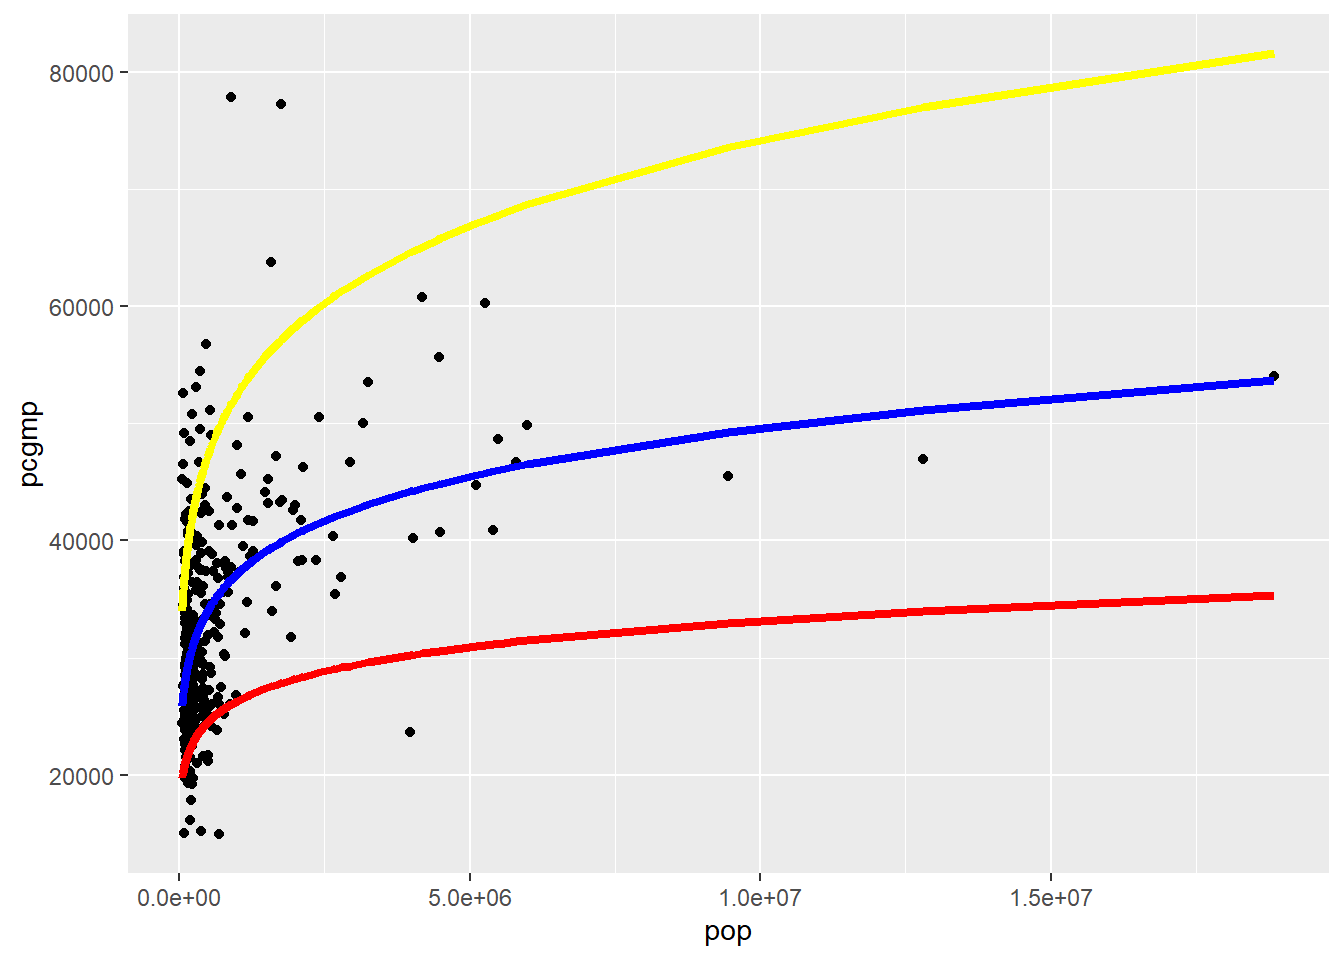
\includegraphics{Homework-03_files/figure-latex/unnamed-chunk-3-1.pdf}

\begin{enumerate}
\def\labelenumi{\arabic{enumi}.}
\setcounter{enumi}{1}
\tightlist
\item
  Write a function, called \texttt{mse()}, which calculates the mean
  squared error of the model on a given data set. \texttt{mse()} should
  take three arguments: a numeric vector of length two, the first
  component standing for \(y_0\) and the second for \(a\); a numerical
  vector containing the values of \(N\); and a numerical vector
  containing the values of \(Y\). The function should return a single
  numerical value. The latter two arguments should have as the default
  values the columns \texttt{pop} and \texttt{pcgmp} (respectively) from
  the \texttt{gmp} data frame from lecture. Your function may not use
  \texttt{for()} or any other loop. Check that, with the default data,
  you get the following
\end{enumerate}

\begin{verbatim}
> mse(c(6611,0.15))
[1] 207057513
> mse(c(5000,0.10))
[1] 298459915
\end{verbatim}

\begin{Shaded}
\begin{Highlighting}[]
\NormalTok{mse=}\ControlFlowTok{function}\NormalTok{(x)\{}
\NormalTok{  a=gmp}\OperatorTok{$}\NormalTok{pcgmp}
\NormalTok{  b=gmp}\OperatorTok{$}\NormalTok{pop}
  \KeywordTok{return}\NormalTok{(}\KeywordTok{mean}\NormalTok{((a}\OperatorTok{-}\NormalTok{x[}\DecValTok{1}\NormalTok{]}\OperatorTok{*}\NormalTok{b}\OperatorTok{^}\NormalTok{x[}\DecValTok{2}\NormalTok{])}\OperatorTok{^}\DecValTok{2}\NormalTok{))}
\NormalTok{\}}
\KeywordTok{mse}\NormalTok{(}\KeywordTok{c}\NormalTok{(}\DecValTok{6611}\NormalTok{,}\FloatTok{0.15}\NormalTok{))}
\end{Highlighting}
\end{Shaded}

\begin{verbatim}
## [1] 207057513
\end{verbatim}

\begin{Shaded}
\begin{Highlighting}[]
\KeywordTok{mse}\NormalTok{(}\KeywordTok{c}\NormalTok{(}\DecValTok{5000}\NormalTok{,}\FloatTok{0.10}\NormalTok{))}
\end{Highlighting}
\end{Shaded}

\begin{verbatim}
## [1] 298459915
\end{verbatim}

\begin{enumerate}
\def\labelenumi{\arabic{enumi}.}
\setcounter{enumi}{2}
\tightlist
\item
  R has several built-in functions for optimization, which we will meet
  as we go through the course. One of the simplest is \texttt{nlm()}, or
  non-linear minimization. \texttt{nlm()} takes two required arguments:
  a function, and a starting value for that function. Run \texttt{nlm()}
  three times with your function \texttt{mse()} and three starting value
  pairs for \(y0\) and \(a\) as in
\end{enumerate}

\begin{Shaded}
\begin{Highlighting}[]
\KeywordTok{nlm}\NormalTok{(mse, }\KeywordTok{c}\NormalTok{(}\DataTypeTok{y0=}\DecValTok{7000}\NormalTok{,}\DataTypeTok{a=}\FloatTok{0.2}\NormalTok{))}
\end{Highlighting}
\end{Shaded}

\begin{verbatim}
## $minimum
## [1] 1168662933
## 
## $estimate
## [1] 6999.9983 -153.6302
## 
## $gradient
## [1] 0 0
## 
## $code
## [1] 1
## 
## $iterations
## [1] 1
\end{verbatim}

\begin{Shaded}
\begin{Highlighting}[]
\KeywordTok{nlm}\NormalTok{(mse, }\KeywordTok{c}\NormalTok{(}\DataTypeTok{y0=}\DecValTok{6611}\NormalTok{,}\DataTypeTok{a=}\FloatTok{0.2}\NormalTok{))}
\end{Highlighting}
\end{Shaded}

\begin{verbatim}
## $minimum
## [1] 1168662933
## 
## $estimate
## [1] 6610.9983 -145.0805
## 
## $gradient
## [1] 0 0
## 
## $code
## [1] 1
## 
## $iterations
## [1] 1
\end{verbatim}

\begin{Shaded}
\begin{Highlighting}[]
\KeywordTok{nlm}\NormalTok{(mse, }\KeywordTok{c}\NormalTok{(}\DataTypeTok{y0=}\DecValTok{6611}\NormalTok{,}\DataTypeTok{a=}\FloatTok{0.15}\NormalTok{))}
\end{Highlighting}
\end{Shaded}

\begin{verbatim}
## $minimum
## [1] 61857061
## 
## $estimate
## [1] 6610.9999997    0.1263182
## 
## $gradient
## [1]   51.76342 -210.18948
## 
## $code
## [1] 2
## 
## $iterations
## [1] 7
\end{verbatim}

What do the quantities \texttt{minimum} and \texttt{estimate} represent?
What values does it return for these? answer:minimum
代表在所给初值下,均方误差所能达到的最小值,estiamte表示在所给初值下,均方误差最小时参数的估计值

\begin{enumerate}
\def\labelenumi{\arabic{enumi}.}
\setcounter{enumi}{3}
\tightlist
\item
  Using \texttt{nlm()}, and the \texttt{mse()} function you wrote, write
  a function, \texttt{plm()}, which estimates the parameters \(y_0\) and
  \(a\) of the model by minimizing the mean squared error. It should
  take the following arguments: an initial guess for \(y_0\); an initial
  guess for \(a\); a vector containing the \(N\) values; a vector
  containing the \(Y\) values. All arguments except the initial guesses
  should have suitable default values. It should return a list with the
  following components: the final guess for \(y_0\); the final guess for
  \(a\); the final value of the MSE. Your function must call those you
  wrote in earlier questions (it should not repeat their code), and the
  appropriate arguments to \texttt{plm()} should be passed on to them.
\end{enumerate}

\begin{Shaded}
\begin{Highlighting}[]
\NormalTok{plm=}\ControlFlowTok{function}\NormalTok{(x,}\DataTypeTok{Y=}\NormalTok{gmp}\OperatorTok{$}\NormalTok{pcgmp,}\DataTypeTok{N=}\NormalTok{gmp}\OperatorTok{$}\NormalTok{pop)\{}
\NormalTok{  result=}\KeywordTok{nlm}\NormalTok{(mse,x)}
\NormalTok{  b=}\KeywordTok{list}\NormalTok{(}\DataTypeTok{y0=}\NormalTok{result}\OperatorTok{$}\NormalTok{estimate[}\DecValTok{1}\NormalTok{],}\DataTypeTok{a=}\NormalTok{result}\OperatorTok{$}\NormalTok{estimate[}\DecValTok{2}\NormalTok{],}\DataTypeTok{final_value=}\NormalTok{result}\OperatorTok{$}\NormalTok{minimum)}
  \KeywordTok{return}\NormalTok{(b)}
\NormalTok{\}}
\end{Highlighting}
\end{Shaded}

What parameter estimate do you get when starting from \(y_0 = 6611\) and
\(a = 0.15\) From \(y_0 = 5000\) and \(a = 0.10\)? If these are not the
same, why do they differ? Which estimate has the lower MSE?\\
answer:因为迭代的初值不同,所以最后收敛的结果也不同, \(y_0 = 6611\) and
\(a = 0.15\)MSE更低

\begin{Shaded}
\begin{Highlighting}[]
\KeywordTok{plm}\NormalTok{(}\KeywordTok{c}\NormalTok{(}\DecValTok{6611}\NormalTok{,}\FloatTok{0.15}\NormalTok{))}
\end{Highlighting}
\end{Shaded}

\begin{verbatim}
## $y0
## [1] 6611
## 
## $a
## [1] 0.1263182
## 
## $final_value
## [1] 61857061
\end{verbatim}

\begin{Shaded}
\begin{Highlighting}[]
\KeywordTok{plm}\NormalTok{(}\KeywordTok{c}\NormalTok{(}\DecValTok{5000}\NormalTok{,}\FloatTok{0.1}\NormalTok{))}
\end{Highlighting}
\end{Shaded}

\begin{verbatim}
## Warning in nlm(mse, x): NA/Inf被换成最大的正值

## Warning in nlm(mse, x): NA/Inf被换成最大的正值

## Warning in nlm(mse, x): NA/Inf被换成最大的正值

## Warning in nlm(mse, x): NA/Inf被换成最大的正值

## Warning in nlm(mse, x): NA/Inf被换成最大的正值

## Warning in nlm(mse, x): NA/Inf被换成最大的正值
\end{verbatim}

\begin{verbatim}
## $y0
## [1] 5000
## 
## $a
## [1] 0.1475913
## 
## $final_value
## [1] 62521485
\end{verbatim}

\begin{enumerate}
\def\labelenumi{\arabic{enumi}.}
\setcounter{enumi}{4}
\tightlist
\item
  \emph{Convince yourself the jackknife can work}.

  \begin{enumerate}
  \def\labelenumii{\alph{enumii}.}
  \tightlist
  \item
    Calculate the mean per-capita GMP across cities, and the standard
    error of this mean, using the built-in functions \texttt{mean()} and
    \texttt{sd()}, and the formula for the standard error of the mean
    you learned in your intro. stats. class (or looked up on
    Wikipedia\ldots).
  \end{enumerate}
\end{enumerate}

\begin{Shaded}
\begin{Highlighting}[]
\KeywordTok{mean}\NormalTok{(gmp}\OperatorTok{$}\NormalTok{pcgmp)}
\end{Highlighting}
\end{Shaded}

\begin{verbatim}
## [1] 32922.53
\end{verbatim}

\begin{Shaded}
\begin{Highlighting}[]
\KeywordTok{sd}\NormalTok{(gmp}\OperatorTok{$}\NormalTok{pcgmp)}\OperatorTok{/}\KeywordTok{sqrt}\NormalTok{(}\KeywordTok{length}\NormalTok{(gmp}\OperatorTok{$}\NormalTok{pcgmp))}
\end{Highlighting}
\end{Shaded}

\begin{verbatim}
## [1] 481.9195
\end{verbatim}

\begin{verbatim}
b. Write a function which takes in an integer `i`, and calculate the mean per-capita GMP for every city _except_ city number `i`.
\end{verbatim}

\begin{Shaded}
\begin{Highlighting}[]
\NormalTok{mean_i=}\ControlFlowTok{function}\NormalTok{(i,}\DataTypeTok{Y=}\NormalTok{gmp}\OperatorTok{$}\NormalTok{pcgmp)\{}
  \KeywordTok{return}\NormalTok{(}\KeywordTok{mean}\NormalTok{(Y[}\OperatorTok{-}\NormalTok{i]))}
\NormalTok{\}}
\end{Highlighting}
\end{Shaded}

\begin{verbatim}
c. Using this function, create a vector, `jackknifed.means`, which has the mean per-capita GMP where every city is held out in turn.  (You may use a `for` loop or `sapply()`.)
\end{verbatim}

\begin{Shaded}
\begin{Highlighting}[]
\NormalTok{n=}\KeywordTok{length}\NormalTok{(gmp}\OperatorTok{$}\NormalTok{pcgmp)}
\NormalTok{jackknifed.means=}\KeywordTok{vector}\NormalTok{(}\DataTypeTok{length =}\NormalTok{ n)}
\ControlFlowTok{for}\NormalTok{ (i }\ControlFlowTok{in} \DecValTok{1}\OperatorTok{:}\NormalTok{n)\{}
\NormalTok{  jackknifed.means[i]=}\KeywordTok{mean_i}\NormalTok{(i)}
\NormalTok{\}}
\end{Highlighting}
\end{Shaded}

\begin{verbatim}
d. Using the vector `jackknifed.means`, calculate the jack-knife approximation to the standard error of the mean.  How well does it match your answer from part (a)?
answer:和(a)中结果一样
\end{verbatim}

\begin{Shaded}
\begin{Highlighting}[]
\KeywordTok{sqrt}\NormalTok{((n}\DecValTok{-1}\NormalTok{)}\OperatorTok{^}\DecValTok{2}\OperatorTok{/}\NormalTok{n}\OperatorTok{*}\KeywordTok{var}\NormalTok{(jackknifed.means))}
\end{Highlighting}
\end{Shaded}

\begin{verbatim}
## [1] 481.9195
\end{verbatim}

\begin{enumerate}
\def\labelenumi{\arabic{enumi}.}
\setcounter{enumi}{5}
\tightlist
\item
  Write a function, \texttt{plm.jackknife()}, to calculate jackknife
  standard errors for the parameters \(y_0\) and \(a\). It should take
  the same arguments as \texttt{plm()}, and return standard errors for
  both parameters. This function should call your \texttt{plm()}
  function repeatedly. What standard errors do you get for the two
  parameters?
\end{enumerate}

\begin{Shaded}
\begin{Highlighting}[]
\NormalTok{plm.jackknife=}\ControlFlowTok{function}\NormalTok{(x,}\DataTypeTok{Y=}\NormalTok{gmp}\OperatorTok{$}\NormalTok{pcgmp)\{}
\NormalTok{  vec_y0=}\KeywordTok{vector}\NormalTok{(}\DataTypeTok{length =}\NormalTok{ n)}
\NormalTok{  vec_a=}\KeywordTok{vector}\NormalTok{(}\DataTypeTok{length =}\NormalTok{ n)}
  \ControlFlowTok{for}\NormalTok{ (i }\ControlFlowTok{in} \DecValTok{1}\OperatorTok{:}\NormalTok{n)\{}
\NormalTok{    vec_y0[i]=}\KeywordTok{plm}\NormalTok{(x,Y[}\OperatorTok{-}\NormalTok{i])}\OperatorTok{$}\NormalTok{y0[}\DecValTok{1}\NormalTok{]}
\NormalTok{    vec_a[i]=}\KeywordTok{plm}\NormalTok{(x,Y[}\OperatorTok{-}\NormalTok{i])}\OperatorTok{$}\NormalTok{a[}\DecValTok{1}\NormalTok{]}
\NormalTok{  \}}
\NormalTok{  result=}\KeywordTok{list}\NormalTok{(}\DataTypeTok{y0_sd=}\KeywordTok{sqrt}\NormalTok{((n}\DecValTok{-1}\NormalTok{)}\OperatorTok{^}\DecValTok{2}\OperatorTok{/}\NormalTok{n}\OperatorTok{*}\KeywordTok{var}\NormalTok{(vec_y0)),}\DataTypeTok{a_sd=}\KeywordTok{sqrt}\NormalTok{((n}\DecValTok{-1}\NormalTok{)}\OperatorTok{^}\DecValTok{2}\OperatorTok{/}\NormalTok{n}\OperatorTok{*}\KeywordTok{var}\NormalTok{(vec_a)))}
  \KeywordTok{return}\NormalTok{(result)}
\NormalTok{\}}
\end{Highlighting}
\end{Shaded}

\begin{enumerate}
\def\labelenumi{\arabic{enumi}.}
\setcounter{enumi}{6}
\tightlist
\item
  The file \texttt{gmp-2013.dat} contains measurements for for 2013.
  Load it, and use \texttt{plm()} and \texttt{plm.jackknife} to estimate
  the parameters of the model for 2013, and their standard errors. Have
  the parameters of the model changed significantly?
\end{enumerate}

\begin{Shaded}
\begin{Highlighting}[]
\NormalTok{gmp_}\DecValTok{2013}\NormalTok{=}\KeywordTok{read.table}\NormalTok{(}\StringTok{"data/gmp-2013.dat"}\NormalTok{)}
\NormalTok{gmp_}\DecValTok{2013}\NormalTok{=gmp_}\DecValTok{2013}\OperatorTok\KeywordTok{mutate}\NormalTok{(}\DataTypeTok{pop=}\KeywordTok{round}\NormalTok{(gmp}\OperatorTok{/}\NormalTok{pcgmp)) }
\KeywordTok{plm}\NormalTok{(}\KeywordTok{c}\NormalTok{(}\DecValTok{6611}\NormalTok{,}\FloatTok{0.15}\NormalTok{),}\DataTypeTok{Y=}\NormalTok{gmp_}\DecValTok{2013}\OperatorTok{$}\NormalTok{pcgmp,}\DataTypeTok{N=}\NormalTok{gmp_}\DecValTok{2013}\OperatorTok{$}\NormalTok{pop)}
\end{Highlighting}
\end{Shaded}

\begin{verbatim}
## $y0
## [1] 6611
## 
## $a
## [1] 0.1263182
## 
## $final_value
## [1] 61857061
\end{verbatim}

\begin{Shaded}
\begin{Highlighting}[]
\KeywordTok{plm.jackknife}\NormalTok{(}\KeywordTok{c}\NormalTok{(}\DecValTok{6611}\NormalTok{,}\FloatTok{0.15}\NormalTok{),}\DataTypeTok{Y=}\NormalTok{gmp_}\DecValTok{2013}\OperatorTok{$}\NormalTok{pcgmp)}
\end{Highlighting}
\end{Shaded}

\begin{verbatim}
## $y0_sd
## [1] 0
## 
## $a_sd
## [1] 0
\end{verbatim}

\end{document}
